% A Readymade beamer presentation template
% Version 1.1
% Relase date: May 2, 2010
% Released at http://www.stattler.com
% by Rifat Jahan

\documentclass{beamer}
%\usecolortheme[named=green]{structure}
\mode<presentation> {
\usetheme{Madrid} % My favorite!
%\usetheme{Boadilla} % Pretty neat, soft color.
%\usetheme{default}
%\usetheme{Warsaw}
%\usetheme{Bergen} % This template has nagivation on the left
%\usetheme{Frankfurt} % Similar to the default with an extra region at the top.
%\usecolortheme{seahorse} % Simple and clean template
%\usetheme{Darmstadt} % not so good
% Uncomment the following line if you want page numbers and using Warsaw theme
% \setbeamertemplate{footline}[page number]
%\setbeamercovered{transparent}
\setbeamercovered{invisible}
% To remove the navigation symbols from the bottom of slides%
\setbeamertemplate{navigation symbols}{} 
}

\usepackage{graphicx}
%\usepackage{bm} 
% For typesetting bold math (not \mathbold)
%\logo{\includegraphics[height=0.6cm]{yourlogo.eps}}
%
\title[Green GLB]{Cooling Aware and Green Geographical Load Balancing}
%
\author{Yizhen Wang}
\institute[Caltech]
{
California Institute of Technology \\
\medskip
{\emph{ywang3@caltech.edu}}
}
\date{\today}
% \today will show current date. 
% Alternatively, you can specify a date.

\begin{document}
%
\begin{frame}
\titlepage
\end{frame}
%
%
\begin{frame}
\frametitle{ResearchTopic \& Motivation}
\begin{block}
{We have increasing number of data centers}

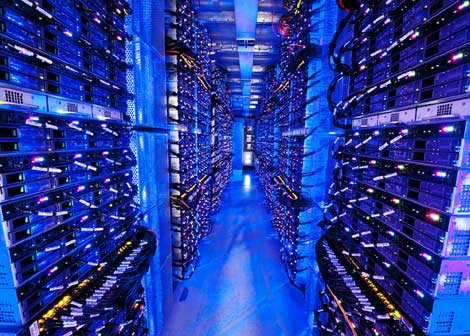
\includegraphics[scale = 0.7]{datacenter.jpg}

\end{block}
\end{frame}
%
%
\begin{frame}
\frametitle{ResearchTopic \& Motivation}
\begin{block}
{We want them to be "green"!}

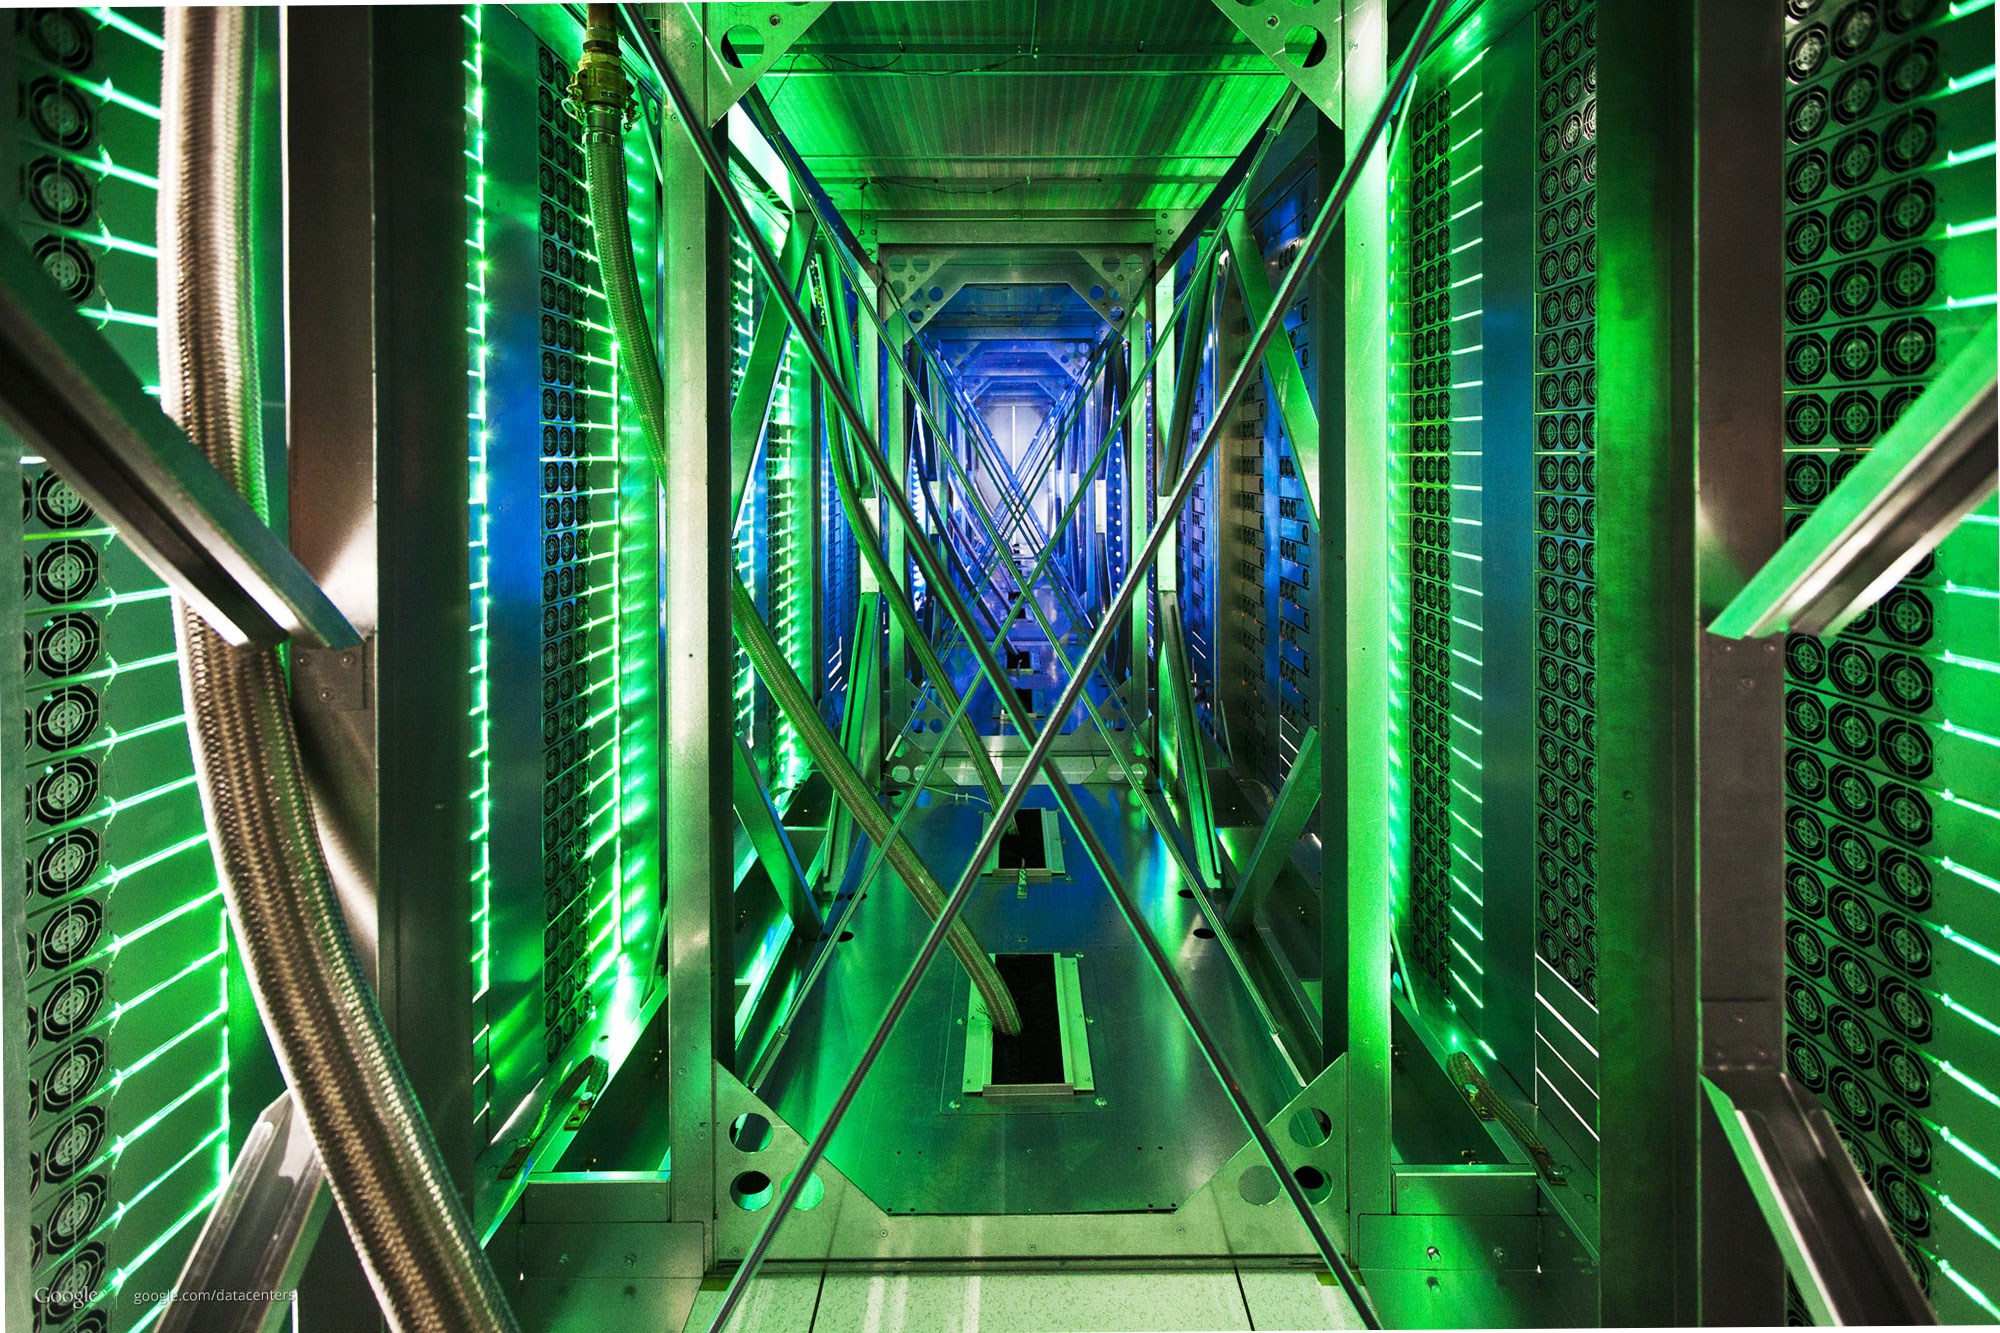
\includegraphics[scale = 0.15]{green.jpg}

\end{block}
\end{frame}
%
%
\begin{frame}
\frametitle{ResearchTopic \& Motivation}
\begin{block}
{We want them to be "green"!}
\begin{itemize}
\item
From firms' point of view, it's always good to cut down the energy cost.
\item
As residents on the earth, we want to be environmental friendly. Sustainability is the key.
\item
It's to everyone's interest to cut brown energy consumption.  
\end{itemize}
\end{block}
\end{frame}
%
%
\begin{frame}
\frametitle{ResearchTopic \& Motivation}
\begin{block}
{We can use renewable energy!}
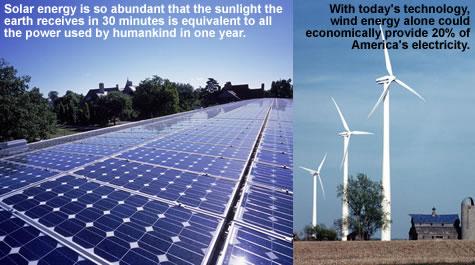
\includegraphics[scale = 0.6]{renewables.jpg}
\end{block}
\end{frame}
%
%
\begin{frame}
\frametitle{ResearchTopic \& Motivation}
\begin{block}
{What's stopping us?}
\begin{itemize}
\item
Installing renewable energy plant is costly.
\item
The output of such plant varies with weather. It's hard to know the right amount of capacity to install. Storage is also needed.
\item
How do we deal the surplus in supply? Sell them? Is selling easy?
\end{itemize}
\end{block}
\end{frame}
%
%
\begin{frame}
\frametitle{ResearchTopic \& Motivation}
\begin{block}
{We believe in Geographical Load Balancing.}
It...
\begin{itemize}
\item
changes the demand curve to fit the supply.
\item
explores the heterogeneity of data center status
\item
causes some unexpected positive side-effect.
\end{itemize}
\end{block}
\end{frame}
%
%
\begin{frame}
\frametitle{ResearchTopic \& Motivation}
\begin{block}
{We believe in Geographical Load Balancing.}
Our work 
\begin{itemize}
\item
for the first time integrates the cooling concerns into the GLB setting, which leads to an actual cut in total energy usage
\item
investigates the environmental impact in terms of carbon emission
\item
compares the performance of using GLB v.s. using storage
\end{itemize}
We yield three major insights:
\begin{itemize}
\item
The cost of running the data center is almost constant across seasons; this potentially solves cooling problem.
\item
The green GLB algorithm is extremely environment friendly
\item
The performance of GLB is comparable to using storage while the cost is much lower.
\end{itemize}
\end{block}
\end{frame}
%
%
\begin{frame}
\frametitle{Experiment Setup}
\begin{block}
{What is a geographical load balancing system?}
\begin{itemize}
\item
Data centers
	\begin{itemize}
	\item
	Has its capacity limit due to no. of server, transmission speed, etc.
	\item
	Has a combination of energy sources.
	\end{itemize}
\item
Source of requests
	\begin{itemize}
	\item
	Where requests are sent out.
	\item
	Set as the population centers.
	\end{itemize}	
\item
Routing in the network
	\begin{itemize}
	\item
	Data/requests transported between source and data center.
	\item
	Need to be carefully planned ahead to minimize cost.
	\end{itemize}
\end{itemize}
\end{block}
\end{frame}

%
%
\begin{frame}
\frametitle{Experiment Setup}
\begin{block}
{Modelling the system}
\begin{itemize}
\item
Renewable availability
	\begin{itemize}
	\item
	How much renewable energy at each data center location?
	\item
	How much of the energy are from wind? from solar?
        \end{itemize}
\item
IT Load
	\begin{itemize}
	\item
	What is the base shape of the load curve?
	\item
	How do we scale it?	
	\end{itemize}
\item
Cooling expenses
	\begin{itemize}
	\item
	What are the cooling options?
	\item
	How do we optimize it?
	\end{itemize}
\item
Cost model
	\begin{itemize}
	\item
	Energy cost
	\item
	Delay cost \& Queuing cost
	\item
	Switch cost
	\end{itemize}

\item
Storage
\end{itemize}
\end{block}
\end{frame}
%
%
\begin{frame}
\frametitle{Experiment Setup}
\begin{block}
{Data centers}
\begin{itemize}
\item
Computation capacity
	\begin{itemize}
	\item
	the capacity is proportional to the no. of servers
	\item
	also depends on how fast the servers are
	\item
	the capacity must be \emph{enough} when there's no GLB.
	\end{itemize}
\item
Cooling equipment
	\begin{itemize}
	\item
	type of cooling: chilled water cooling and air cooling
	\item
	charateristics of each cooling method
	\item
	model the cooling capacity
	\end{itemize}
\end{itemize}
\end{block}
\end{frame}
%
%
\begin{frame}
\frametitle{Experiment Setup}
\begin{block}
{Renewable Availability}
\begin{itemize}
\item
Weather factor
	\begin{itemize}
	\item
	Wind speed, solar irradiance
	\end{itemize}
\item
Time factor
	\begin{itemize}
	\item
	Sunrise/sunset
	\end{itemize}
\item
Scaling to data center's need!
	\begin{itemize}
	\item
	the national aggregate demand/supply ratio
	\end{itemize}
\end{itemize}
\end{block}
\end{frame}
%
%
\begin{frame}
\frametitle{Experiment Setup}
\begin{block}
{IT Load}
\begin{itemize}
\item
Base shape of the curve
	\begin{itemize}
	\item
	we use real traces from HP data center
	\end{itemize}
\item
Scale \& shift
	\begin{itemize}
	\item
	we shift the curve according to timezone and scale it by the population.
	\end{itemize}
\end{itemize}
\end{block}
\end{frame}
%
%
\begin{frame}
\frametitle{Experiment Setup}
\begin{block}
{Cooling}
\begin{itemize}
\item
Air cooling is ideal when outside air is cold.
\item
Chilled water cooling incurs almost constant cost in all circumstances
\item
The no. of servers that need cooling is proportional to the load.
\end{itemize}
\end{block}
\end{frame}
%
%
\begin{frame}
\frametitle{Experiment Setup}
\begin{block}
{Cost}
\begin{itemize}
\item
Energy Cost
	\begin{itemize}
	\item
	Renewable energy is free; grid energy is not.
	\item
	Both computation and cooling needs energy!
	\end{itemize}
\item
Delay Cost \& Queuing Cost
	\begin{itemize}
	\item
	Delay cost is due to transmission b/w data center and the population center.
	\item
	Queuing cost is due to the waiting at data center.
	\end{itemize}
\item
Switch Cost
	\begin{itemize}
	\item
	We don't want to switch on/off machines too often.
	\end{itemize}
\end{itemize}
\end{block}
\end{frame}

\begin{frame}
\frametitle{Experiment Setup}
\begin{block}
{Cost}
\begin{itemize}
\item
The eventual cost model is:
\begin{align*}
\min_{\bf{x}(t), \bf{\lambda}(t)} & \sum_{i \in \mathcal{N}} p_i(l(x_i(t)) + c(x_i(t)) - r_i(t) - e_i(t))^+ \\
& + \sum_{j \in \mathcal{J}}\sum_{i \in \mathcal{N}}
\lambda_{ij}(t)\left(\frac{1}{\mu_i - \lambda_i(t)/x_i(t)} + d_{ij}\right) \\
& + \beta(x_i(t+1) - x_i(t))^+
\end{align*}
\end{itemize}
\end{block}
\end{frame}
%
%
\begin{frame}
\frametitle{Experiment Setup}
\begin{block}
{Constraints}
\begin{itemize}
\item
We impose the necessary real world constraints.
\begin{align*}
& \sum_{i\in \mathcal{N}}\lambda_{ij}(t) = L_j(t), &\forall j\in J  \\
& \lambda_{ij} \geq 0, & \forall i\in N, j\in J  \\
& 0 \leq x_i(t) \leq X_i, & \forall i \in N  \\
& \lambda_i(t) \leq x_i(t)\mu_i & \forall i \in N \\
& 0 \leq es_i(t) \leq ES_i & \forall i \in N \\
& e_i(t) = es_i(t) - es_i(t+1) & \forall i \in N
\end{align*}
\end{itemize}
\end{block}
\end{frame}
%
%
\begin{frame}
\frametitle{Experiment Setup}
\begin{block}
{What is so nice about this model?}
\begin{itemize}
\item
We can use convex optimization technique to solve it!
\end{itemize}
\end{block}
\end{frame}
%
%
\begin{frame}
\frametitle{Experiment Result}
\begin{block}
{Cost saving}
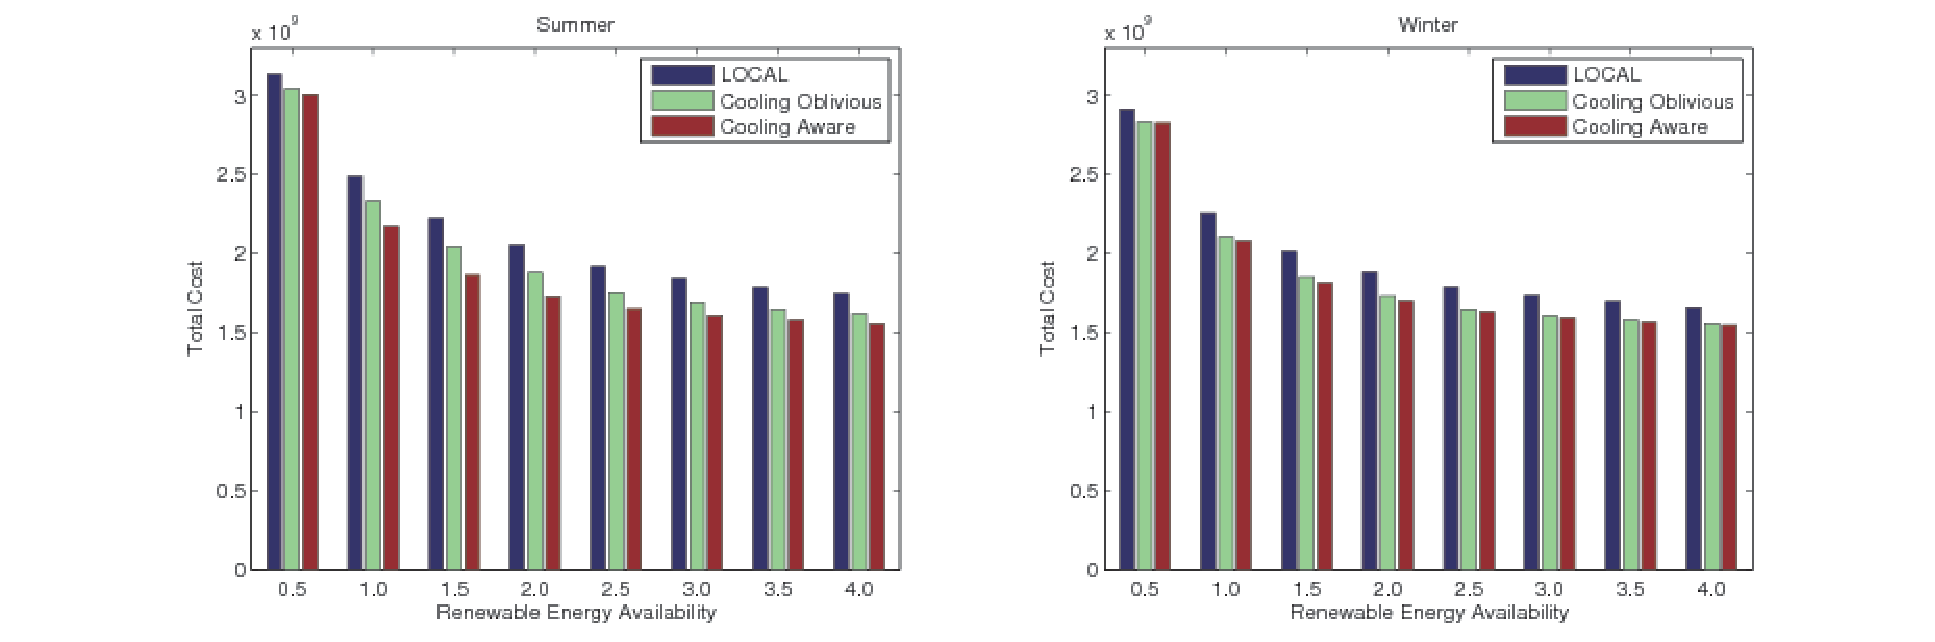
\includegraphics[scale = 0.37]{cost_comparison.pdf}
\end{block}
\end{frame}
%
%
\begin{frame}
\frametitle{Experiment Result}
\begin{block}
{Seasonality}
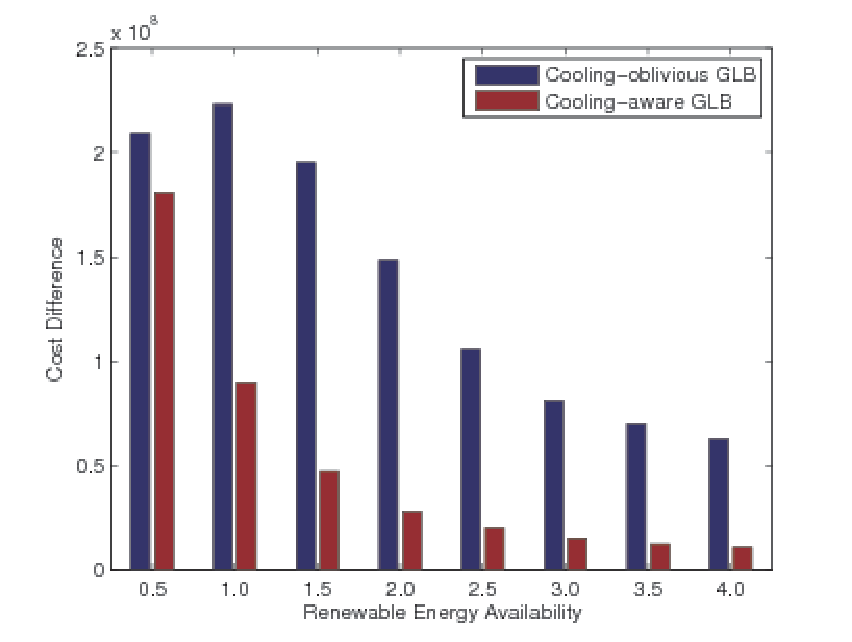
\includegraphics[scale = 0.5]{cost_diff.pdf}
\end{block}
\end{frame}
%
%
\begin{frame}
\frametitle{Experiment Result}
\begin{block}
{Carbon Emission}
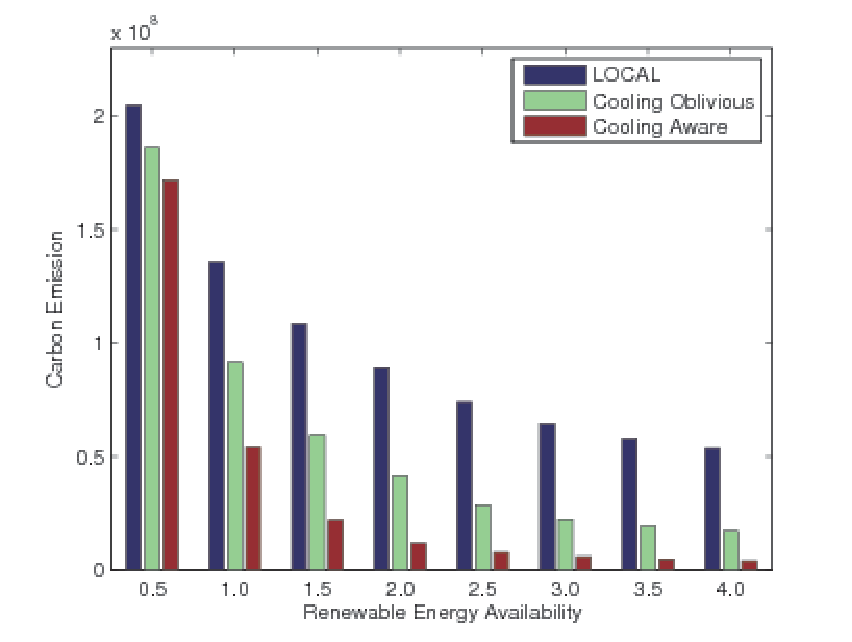
\includegraphics[scale = 0.5]{carbon_summer.pdf}
\end{block}
\end{frame}
%
%
\begin{frame}
\frametitle{Experiment Result}
\begin{block}
{vs Storage}
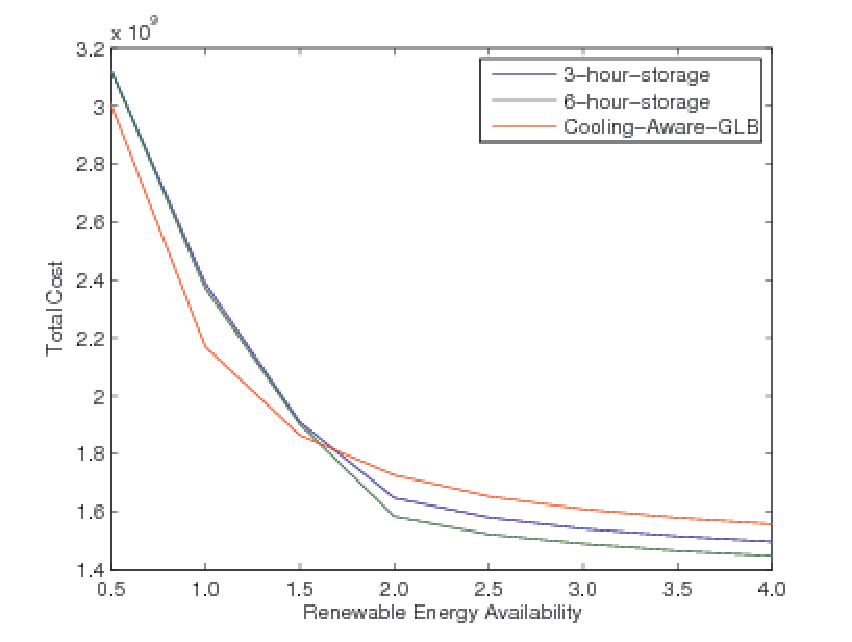
\includegraphics[scale = 0.5]{cost_storage.pdf}
\end{block}
\end{frame}
%
%
\begin{frame}
\frametitle{Experiment Result}
\begin{block}
{vs Storage}
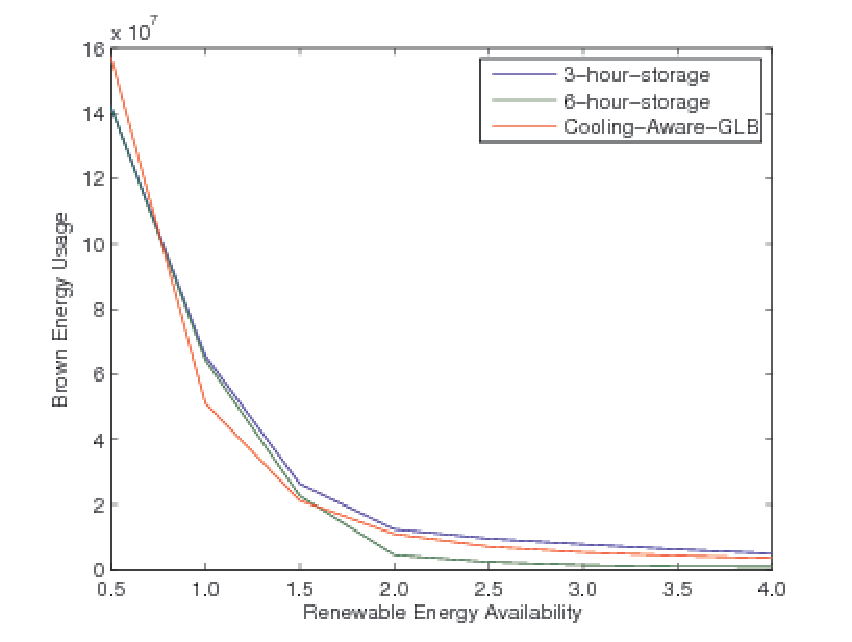
\includegraphics[scale = 0.5]{brown_storage.pdf}
\end{block}
\end{frame}
%
%
\begin{frame}
\frametitle{Future Work}
\begin{block}
{We can still improve}
\begin{itemize}
\item
the online algorithm
	\begin{itemize}
	\item
	involves prediction, needs to be close the optimal.
	\end{itemize}
\item
dynamic pricing
	\begin{itemize}
	\item
	involves changing energy price, which is the general case.
	\end{itemize}
\end{itemize}
\end{block}
\end{frame}
\end{document} 
